\documentclass{article}
\usepackage{listings}
\usepackage{graphicx}

\newcommand{\SolutionName}{Chunker}
\newcommand{\ProjectName}{Chunker}

\newcommand{\code}[1]{\lstinline{#1}}

\title{\ProjectName{} Example}
\date{}


\begin{document}
\maketitle
\begin{abstract}
This example shows how to use invariants to explicate implicit
assumptions in data structures and how they allow one to satisfy
contracts on other APIs, such as System.String.
\end{abstract}

\newcommand\codefamily\sffamily
\lstset{language={[Sharp]C},mathescape=true,flexiblecolumns=true,morekeywords={Requires,Ensures,Invariant},basicstyle=\codefamily\small,literate={->}{{$\rightarrow$}}{2}{<<}{{$\langle$}}{2}{>>}{{$\rangle$}}{2}{!}{{\textbf{!}}}{2},frame=lines,moredelim=[is][\itshape]{@}{@},captionpos=b,numberstyle=\tiny,stepnumber=1,numbersep=2pt}

\section{Adding the Contract Library Reference}
If you are using Visual Studio 2008, or if you for 
some reason want to target a pre-v4 .NET runtime, then you need to:
\begin{itemize}
\item Change the target framework of the project.
\item Manually add a reference to Microsoft.Contracts.dll
\end{itemize}
Otherwise, you may skip this section and go directly the next section!

To add the reference, open the
\textsf{\SolutionName{}} solution and right-click on
\textsf{References} in the \textsf{\ProjectName{}} project and
select \textsf{Add Reference}. Find the \textsf{Microsoft.Contracts}
library in the \textsf{.NET} tab as shown below and click OK.
\begin{center}
  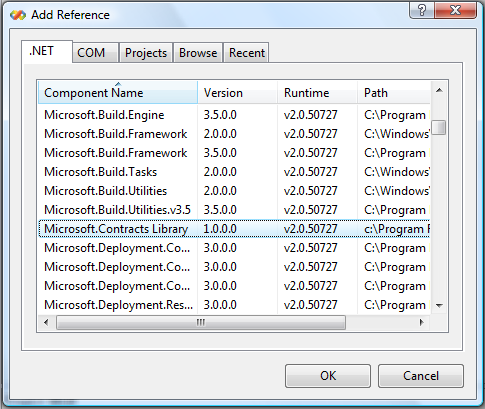
\includegraphics[width=.7\columnwidth]{../Common/addRef.png}
\end{center}



\section{Enabling Static Checking}
\label{sec:start}

After adding the proper reference, go to the Properties of project
\textsf{\ProjectName}, select the Code Contracts pane (at the bottom), and enable static
checking by clicking on the static checking box. Also enable non-null
checking if you wish.
\begin{center}
  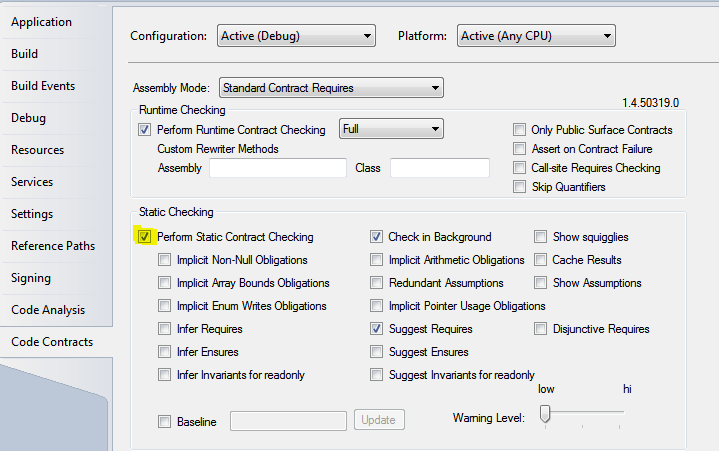
\includegraphics[width=.8\columnwidth]{pane.png}
\end{center}

\section{Overview}
The \code{Chunker} class provides a way to split a string into equal size
sub-strings, each holding a fixed number (chunkSize) of
characters. The chunks are obtained by repeated calls to \code{NextChunk}

A chunker object holds on to the original string in
\code{stringData}. This value is never modified. The size of each
chunk is stored in \code{chunkSize} and also does not vary over the
running time. Finally, \code{returnedCount} holds the number of
characters returned from \code{stringData} so far. Alternatively, we
can think of it as the index into \code{stringData} at which to return
the next chunk.

\section{First Attempt}
Build the example. The build should succeed. After a
moment\footnote{The static checker runs in the background after the regular build.}, 
the static checker should warn about the call to \code{Substring} in \code{NextChunk}.
\begin{center}
  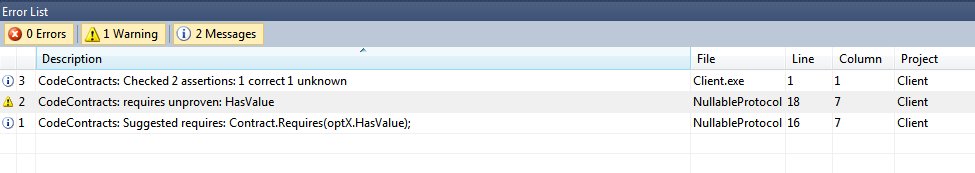
\includegraphics[width=1\columnwidth]{errors1.png}
\end{center}
The documentation (and our corresponding contracts) on
\code{String.Substring(int,int)} state that \code{startIndex +
length} must be within the string extent. Furthermore,
\code{startIndex} and \code{length} must be non-negative.

The Chunker code written so far does not guarantee these
conditions. E.g., the caller to the constructor could provide a
non-positive chunkSize. Similarly, nothing is known about the relation
between \code{stringData.Length} and \code{returnedData}.

\section{Writing the Object Invariant}
Let's write an object invariant that makes these relations
explicit. In the Chunker class, at the member level, type \code{cim
  TAB TAB} to get an emtpy object invariant declaration:
\begin{center}
  \includegraphics[width=.5\columnwidth]{objinv1.png}
\end{center}
Now fill in the first invariant, stating that \code{chunkSize} is
positive (we don't want 0, as there are an infinite number of 0
length chunks we could extract).
\begin{lstlisting}
Contract.Invariant(chunkSize > 0);
\end{lstlisting}
Under this invariant, write \code{ci TAB TAB} to get another empty
invariant and fill it in to specify that \code{returnedCount} is
similarly non-negative.
\begin{lstlisting}
Contract.Invariant(returnedCount >= 0);
\end{lstlisting}
Add one more invariant, specifying that \code{returnedCount}
is never more than the string length.
\begin{lstlisting}
Contract.Invariant(returnedCount <= stringData.Length);
\end{lstlisting}
Finally, for good measure, let's also add the invariant that 
\code{stringData} should never be null.
\begin{lstlisting}
Contract.Invariant(stringData != null);
\end{lstlisting}
In fact, you should add this invariant \emph{before} the invariant
accessing \code{stringData.Length}, otherwise the checker will
complain, and you might get a runtime null reference exception.
Your object invariant should now look as follows:
\begin{center}
  \includegraphics[width=.8\columnwidth]{objinv2.png}
\end{center}

\section{Establishing the Object Invariant}
If you build again, you see that the checker emits a new set of warnings:
\begin{center}
  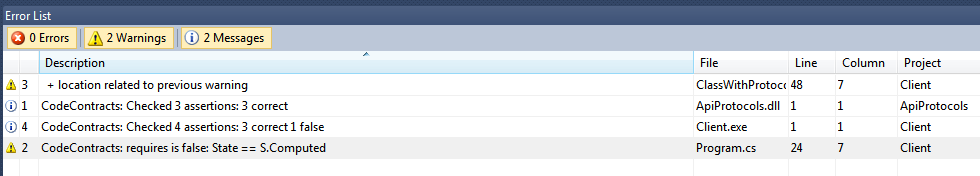
\includegraphics[width=1\columnwidth]{errors2.png}
\end{center}
The two pre-conditions that \code{length} and \code{startIndex} must be non-negative
are now satisfied in \code{NextChunk}. Before focusing on the
remaining issue calling \code{Substring}, let's look at the
constructor of Chunker. The checker warns that we may not establish
the object invariant by the end of the constructor. In fact the first
two messages suggest how to make sure we do, by adding the following
pre-conditions to the Chunker constructor:
\begin{lstlisting}
Contract.Requires(chunkSize > 0);
Contract.Requires(source != null);
\end{lstlisting}
Remember to use the shortcuts (cr TAB TAB for a general requires
and crn TAB TAB for non-null requires).

\section{Handling Border Cases}
If you rebuild the project after adding the requires to the
constructor, we should see the following remaining problem in \code{NextChunk}:
\begin{center}
  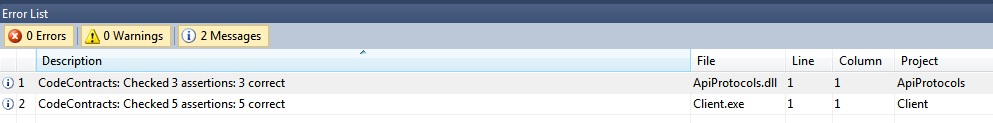
\includegraphics[width=1\columnwidth]{errors3.png}
\end{center}
The checker is complaining that \code{returnedCount} might be bigger
than  \code{stringData.Length - chunkSize}.
Of course, this situation
may arise when we get near the end of the string. In that case, there
may not be enough characters left. To fix this problem, we can change
the code as follows:
\begin{lstlisting}
    public string NextChunk()
    {
      string s;
      if (returnedCount <= stringData.Length - chunkSize)
      {
        s = stringData.Substring(returnedCount, chunkSize);
      }
      else
      {
        s = stringData.Substring(returnedCount);
      }
      returnedCount += s.Length;
      return s;
    }
\end{lstlisting}
Now the checker should not issue any further warnings.

The solution contains the file ChunkerFinal.cs (not compiled) that
contains the final code and contracts.
\end{document}
